\documentclass[10pt,journal,compsoc]{IEEEtran}
\usepackage[dvipsnames]{xcolor}
\usepackage{cite}
\usepackage{amsmath,amssymb,amsfonts}
\usepackage{algorithmic}
\usepackage{graphicx}
\usepackage{textcomp}
\usepackage{url}
\usepackage{caption}
\usepackage{subcaption}

\usepackage{colortbl}

\def\UrlBreaks{\do\/\do-}
\begin{document}
%
% paper title
% Titles are generally capitalized except for words such as a, an, and, as,
% at, but, by, for, in, nor, of, on, or, the, to and up, which are usually
% not capitalized unless they are the first or last word of the title.
% Linebreaks \\ can be used within to get better formatting as desired.
% Do not put math or special symbols in the title.
	%\title{Bare Demo of IEEEtran.cls for\\ IEEE Computer Society Journals}
%
\title{Overtaking Uncertainty with Evolutionary TORCS controllers:
  Combining BLX with Decreasing $\alpha$ Operator and Grand Prix Selection}

\author{Mohammed~Salem, Antonio~M.~Mora, Juan~J.~Merelo% <-this % stops a space
\IEEEcompsocitemizethanks{\IEEEcompsocthanksitem M. Salem was with the Department of Computer Sciences, University of Mascara, Algeria.\protect\\
% note need leading \protect in front of \\ to get a newline within \thanks as
% \\ is fragile and will error, could use \hfil\break instead.
E-mail: salem@univ-mascara.dz
\IEEEcompsocthanksitem A~M.~Mora was with the Department of Signal Theory, Telematics and Communications, ETSIIT-CITIC, University of Granada, Spain.\protect\\
Email: amorag@ugr.es
\IEEEcompsocthanksitem J~J.~Merelo was with the Department of Computer Architecture and Computer Technology. University of Granada, Spain.\protect\\
Email: jmerelo@ugr.es
}% <-this % stops an unwanted space
\thanks{Manuscript received December XX, 2019; revised XXXX, 2020.}}


\IEEEtitleabstractindextext{%
  \begin{abstract}
    Evolution is a powerful problem-solving technique, extensively
used for designing racing car controllers, but with a series of
challenges: an evaluation function that can separate the best
controllers from the rest, and a series of operators that can explore
different possibilities in the controller search space. Within the
context of the TORCS racing simulator, in this paper, we introduce a
selection policy based on competition and called
\textit{Grand Prix Selection} (GPS), which will be able to increase
robustness by using something more realistic than solo race scores to
select individuals. Additionally, we increase the exploitative power
of this kind of selection via a BLX operator with continuously
decreasing $alpha$. We compare these new selection and operator with
hybrid approaches that apply GPS only part of the time, as well as
other classical crossover operators. In general, experiments show that
these combined improvements establish a new level of performance of
evolved controllers, being able to beat, both standard and previously
evolved ones, as well as a high-ranked controller of TORCS
competitions.
\end{abstract}

% Note that keywords are not normally used for peerreview papers.
\begin{IEEEkeywords}
Simulated Car Racing, TORCS, Fuzzy Controllers, Autonomous
controllers, Genetic Algorithms, Optimization, BLX-$\alpha$ Crossover,
Grand Prix Selection, Uncertainty, Competitive fitness
\end{IEEEkeywords}}

% make the title area
\maketitle


\IEEEdisplaynontitleabstractindextext
\IEEEpeerreviewmaketitle



\IEEEraisesectionheading{\section{Introduction}\label{sec:introduction}}

Driving a simulated car can be formulated as an optimization problem in which you have to map inputs that include data about the driving environment as well as car data, to the output: throttling and steering. This mapping has 
 to meet a series of standards: cars should not crash and should have a
reasonable speed \cite{Autodriv2006}. Additionally, in a racing car, the controller has to be designed so that the car wins in as many races as possible.

Since there are so many variables in this problem, the search space is usually reduced using heuristic rules. For instance, deciding the type of controller is usually done before the design process begins, and a single, parametrized one
is chosen; fixed rules, as well as neural networks \cite{KIM201287} or fuzzy controllers \cite{PerezEvolvingFuzzy09}, are often used. 
Additionally, training (or learning) \cite{Loiacono:2012:LEA:2212908.2212953} can be done online (during the
race), so that it can adapt itself to new and previously unseen,
scenarios and competitors, or it can be fixed training offline. 

We have been using genetically-optimized fuzzy controllers in this line of work, with increasing success \cite{salem_evo17},\cite{salem_evo18}.
However, in a simulated and realistic racing car environment like the one we use, racing car scores are a
    statistical variable whose value will vary depending on the track and
    (simulated) atmospheric conditions; and we should never forget
    that score in a training track will always be a surrogate of its
    actual score when racing against other cars on different tracks,
    which adds another layer of uncertainty, making this a {\em noisy} optimization problem.
If training is done before the
    race, and the controllers are fixed via an optimization process,
    the uncertainty in the evaluation of every controller will make
    the resulting score in unknown tracks with unknown rivals
    uncertain at best.

A potentially useful way to increase robustness, that
is, reduce uncertainty is to make the evaluation process
as close as possible to the environment in which the controller will
eventually compete, in a race with other competitors. Hereafter, we will use in general the
  terminology ``reduce uncertainty'' to mean that we attend to increase the robustness of the result, that is, obtain results whose
  performance is not affected by the selection procedure and that are
  consistently good performing. However, robustness is something that
  cannot be measured or appreciated directly, which is why we will
  refer to uncertainty and its reduction in the rest of the paper.

If we can eliminate individually-computed fitness and move to an
environment where fitness is only a relative value, that is, can only
be computed relatively to other individuals, we will be avoiding one
source of uncertainty. We accomplish this by substituting a single
(and uncertain) fitness by a {\em podium} (a ranking after several races
against other opponents) in which car controllers that win the most
races will proceed to the next generation, while those that do not,
will simply be removed from the pool. We can further reduce
uncertainty even more by repeating races several times."  By doing
this, we try to overcome one of the biggest challenges we have found
in this line of research. Uncertainty in selection was already
identified as such in its first paper \cite{salem_evo17}, which
introduced a basic fuzzy-controller based car driving system. This
system was iteratively improved in \cite{salem_evo18,salem_cig2018},
by using an EA to change the shape and values of the fuzzy
controllers. However, we still had to deal with uncertainty, as well
as a suboptimal exploration of the parameter space; the main issue was
that we were using a surrogate to measure the performance of the bot
by doing solo races, and we tried to make that surrogate as accurate
as possible by testing different fitness functions, but also, in
\cite{salem_cig2018}, by racing the best individuals in the last
generation. Introducing races in the selection of the ``winner'', even
if it was in the last generation, improved results, so this kind of
competitive selection was extended by introducing real races from
every few generations in \cite{DBLP:conf/cig/SalemMG19}, where we also
applied the BLX-$alpha$ operator, and checked two different
configurations using a fixed and a decreasing $\alpha$. This operator
combines exploration and exploitation and lets the designer establish
the balance between both factors in the search. The results with
decreasing $\alpha$ were the best obtained so far. Although this
additional operator, by itself, did not reduce uncertainty in the
selection of individual car controllers, by enhancing search
capabilities it made possible accessing parts of the search space
where controllers with low uncertainty could be found.

Thus, in this paper we are testing the best approaches we have found
all together in an algorithm, considering a kind of selection based on
comparisons of performance, which we have called \textit{Grand Prix Selection}
(GPS). Although this selection uses a score that could be assimilated
to a fitness, it is actually an extension of a tournament selection
policy since it creates tournaments of several individuals, and
``scores'' them according to how they fare in these races. This is not
a fitness, since it is not intrinsic to the individual. It is indeed
equivalent to, an $n$-tournament selection that is repeated several
times, giving a score of $n$ to the first, $n-1$ to the second, and
then using this for selection. That score is, thus, not a fitness but
a way of keeping track of the position of the individual in the
different tournaments it has participated; since, in this context, we
have no way of evaluating (i.e. assigning a fitness) to a controller
but only a way to compare them, this approach has been denominated in
ocassions {\em
fitnessless}, as it was called, for instance, in
\cite{jaskowski2008winning}.  This selection policy is combined with
other policies or by itself, is the only way for car controllers to be
selected for the next generation.

This work also presents an exhaustive study, where we have checked how
this Grand Prix Selection works compared with mixed competition- and
fitness-based races, or simply using a selection for those controllers
that have the highest fitness in the last generation.  This reduction
of uncertainty has been proved also to reduce diversity in the genetic
pool \cite{DBLP:journals/tcci/MereloLFGCCRMGTCC16}, which is why the
introduction of the \mbox{BLX-$\alpha$} operator, with a certain
explorative component, achieves better results than GPS by itself, as
we will show here.  Besides, we have compared the influence of the
\mbox{BLX-$\alpha$} operator on the performance of the evolved
controllers with others using standard crossover operators, since we
aim to better control the diversity in the population.

The rest of the paper is organized as follows. Next, we present the
state of the art, to be followed by a description of the TORCS
simulator and the previously defined fuzzy controllers in Section
\ref{sec:methods}. After this, the evolutionary algorithm implemented
is explained in Section \ref{sec:ga}, including an extensive explanation of the new selection policy as well as the BLX-$\alpha$ crossover operator. After it, the experiments conducted and the obtained results are described in
Section \ref{sec:results}. Finally, conclusions and future lines of
work will be presented in Section \ref{sec:conclusions}. 





%%%%%%%%%%%%%%%%%%%%%%%%%%%%%%  STATE OF THE ART  %%%%%%%%%%%%%%%%%%%%%%%%%%%%%%
\section{State of the Art}
\label{sec:soa}

The problem of designing controllers for racing cars has been
approached using soft computing since the first papers were
published; however, they differ in the way the specific controlled
works. In many cases, they learn during the race; reinforcement
learning has that specific capability, and it was used by Loiacono et
al. \cite{loiacono2010learning} in the first paper that uses it. It is still one of the most popular methods, as is shown in recent papers like \cite{remondaformula,waghdistributed}.

However, it is not the only kind of soft computing method
used. \cite{mirus2019short} uses a neuromorphic architecture, namely,
spiking neural networks, but using, the same way we do in our works, a single track for training. The kind of data used for the design of racing cars is
also different depending on the author. 
According to our previous works \cite{salem_evo17},\cite{salem_evo18},\cite{salem_cig2018}, in general, successful racing could be achieved using only these sensor values to drive the car, since they give enough information to avoid collisions, drive as close as possible to the center of the track, and drive as fast as possible.

Other soft computing methods have been combined also with evolutionary algorithms on several occasions, such as \cite{10.1371/journal.pone.0213193} which uses neuroevolution. Thus, controllers trained in one track are briefly re-trained for use in other tracks, in what is called ``transfer learning''. This is also the technique applied by the authors in \cite{verma2018programmatically}. 


%%%%%%%%%%%%%%%%%%%%%%%%%%%%%% TORCS  %%%%%%%%%%%%%%%%%%%%%%%%%%%%%%

All the different approaches would not have been possible without a
racing car simulator that could be the testbed for them all, which was
TORCS (The Open Racing Car Simulator) \cite{torcs4}. The TORCS racing simulator
continues to be one of the main platforms for testing different autonomous driving or bot creation strategies. Only in the last year (2019) there are around 200 articles that mention TORCS; \cite{badue2019selfdriving} revises its applications for the last 20 years. It can be considered as the most successful platform used for this kind of problem.

Fuzzy controllers are considered in around 15\% of the aforementioned articles, while around 30\% mentions evolutionary algorithms; very few, however, around 7\%, use both, and most of them are not actually using TORCS (but just mentioning it); so the approach in this line of research is truly original in this context.

There are several possible approaches to autonomous driving and its
solution using TORCS, such as neural networks or reinforcement learning \cite{abuzekry2comparative}. 
You can also use vision to have a more complete, although a more complicated, view of where the car is and where it is going, or just use sensors, which on one hand check the most immediate scenario, but on the other hand are more precise and easy to process.

In our case, we have opted for the latter, although other authors like Zhu et al. \cite{zhu2019vision} rather
consider vision, using TORCS as a testbed for a different kind of
algorithms. On the other hand \cite{8833873} uses deep learning, working with real images instead of sensor values, whereas \cite{Kaushik_2018_ECCV_Workshops} describes a DDPG (deep deterministic policy gradient), that uses images to learn behaviors for specific racing scenarios.

TORCS, being a realistic simulator, can introduce `noise' into the
track conditions, so that races will never be the same. In general,
this is the case for most games: there are sources of uncertainty
either in the game environment itself or in the behavior of
non-playing characters that act as adversaries in the game; the game
bot or controller itself can also have non-deterministic rules, which
is an additional source of uncertainty. Plus games are games, and the
best way of checking how well a bot or controller plays, is by playing
the game. This way of evolving bots was called {\em fitnessless
coevolution}, and was defined in
\cite{Jaskowski:2008:FC:1389095.1389161}. This is a precedent to Grand
Prix Selection, presented here, whose essence is to get rid of a
fitness score resulting from the evaluation of an individual,
substituting it with a score obtained by the controller in more
realistic competitive conditions.

The concept, however, goes back at least to
\cite{Angeline:1993:CEE:645513.657590}, which calls it a ``competitive
fitness environment''. Fitnessless evolution was further developed in
\cite{rosin1995methods}, but it has been also used in genetic
programming by Tettamanzi in \cite{tettamanzi1996genetic}.

However, the competitions played in those works were not, strictly,
games. Selection based on competition has been used in games extensively, like
\cite{Jaskowski2008,10.1007/978-3-540-78671-9_2,fernandez2016_only_one}.
Deriving which individuals are the best from these races, taking into account
the {\em noisy} environment we have mentioned, is not trivial
either. As recently as 2017, an ELO-based ranking strategy was
introduced for selecting winning bots in a fighting game
\cite{7792145}. The first one mentions ``imperfect information'',
precisely, as one of the factors to use this competition-based selection strategy.

Since we are working with racing games, we will introduce a score that
is closer to the one used in that kind of game. This will be
presented after the rest of the methods and tools used in this paper. 


%%%%%%%%%%%%%%%%%%%%%%%%%%%%  METHODS  %%%%%%%%%%%%%%%%%%%%%%%%%%%%

\section{Methods and tools}
\label{sec:methods}

This section presents the environment where the study has been conducted, i.e. the simulator TORCS, as well as the fuzzy sub-controllers designed in previous works and which will be the `target' of the optimization process conducted in this paper. 

%-------------------------------  TORCS ----------------------------
%

\subsection{Simulation environment}

\begin{figure}[!ht] 
	\begin{center}
		\includegraphics[scale=0.26]{fig/torcs-sensors}
		\caption {TORCS capture showing some of the sensors
                used by the autonomous drivers (controllers). Figure from \cite{DBLP:conf/cig/SalemMG19}.}
		\label{fig:torcs-sensors}
	\end{center}
\end{figure}


We are using in this study The Open Racing Car Simulator (TORCS) \cite{torcs4}, which is free software and offers realistic physics, as well as telemetry that is used by the car controllers to gauge their position with respect to the track, the position of the rest of the players, and self-measurements like speed, damage incurred or angle. These measurements are connected to car sensors \cite{torcs5}, which are represented in Figure \ref{fig:torcs-sensors}. TORCS provides these sensor values as input to the car controller and these will be
used to manage the car by means of actuators such as brake, accelerator, steering wheel, or gearbox. 
This simulator has been used in many other studies in the area of autonomous driving or simulated racing car evolution.
Other open-source simulators, mentioned in \cite{Loiacono:2012:LEA:2212908.2212953}, are also available: VDrift
if more focused on 3D realism, and Speed Dreams is  a fork of
TORCS, same as Gym-TORCS, which is a Python wrapper which is specially designed to test controllers based on reinforcement learning.

Although our results are not TORCS specific, we have been
working on this since it has got all the telemetry and simulation
tools that we need, and besides it has been repeatedly used in
competitions, so it is a good testbed to evaluate the performance of new controllers, in case the competitions came back.

TORCS does not impose a specific way for programming the controllers;
it can be done via any system that maps inputs to outputs. We decided
to use fuzzy sub-controllers.

%---------------------------  FUZZY SUB-CONTROLLERS ----------------------------

\subsection{Fuzzy sub-controllers}
\label{subsec:fuzzy-controllers}

\begin{figure}[!ht]
  \begin{center}
    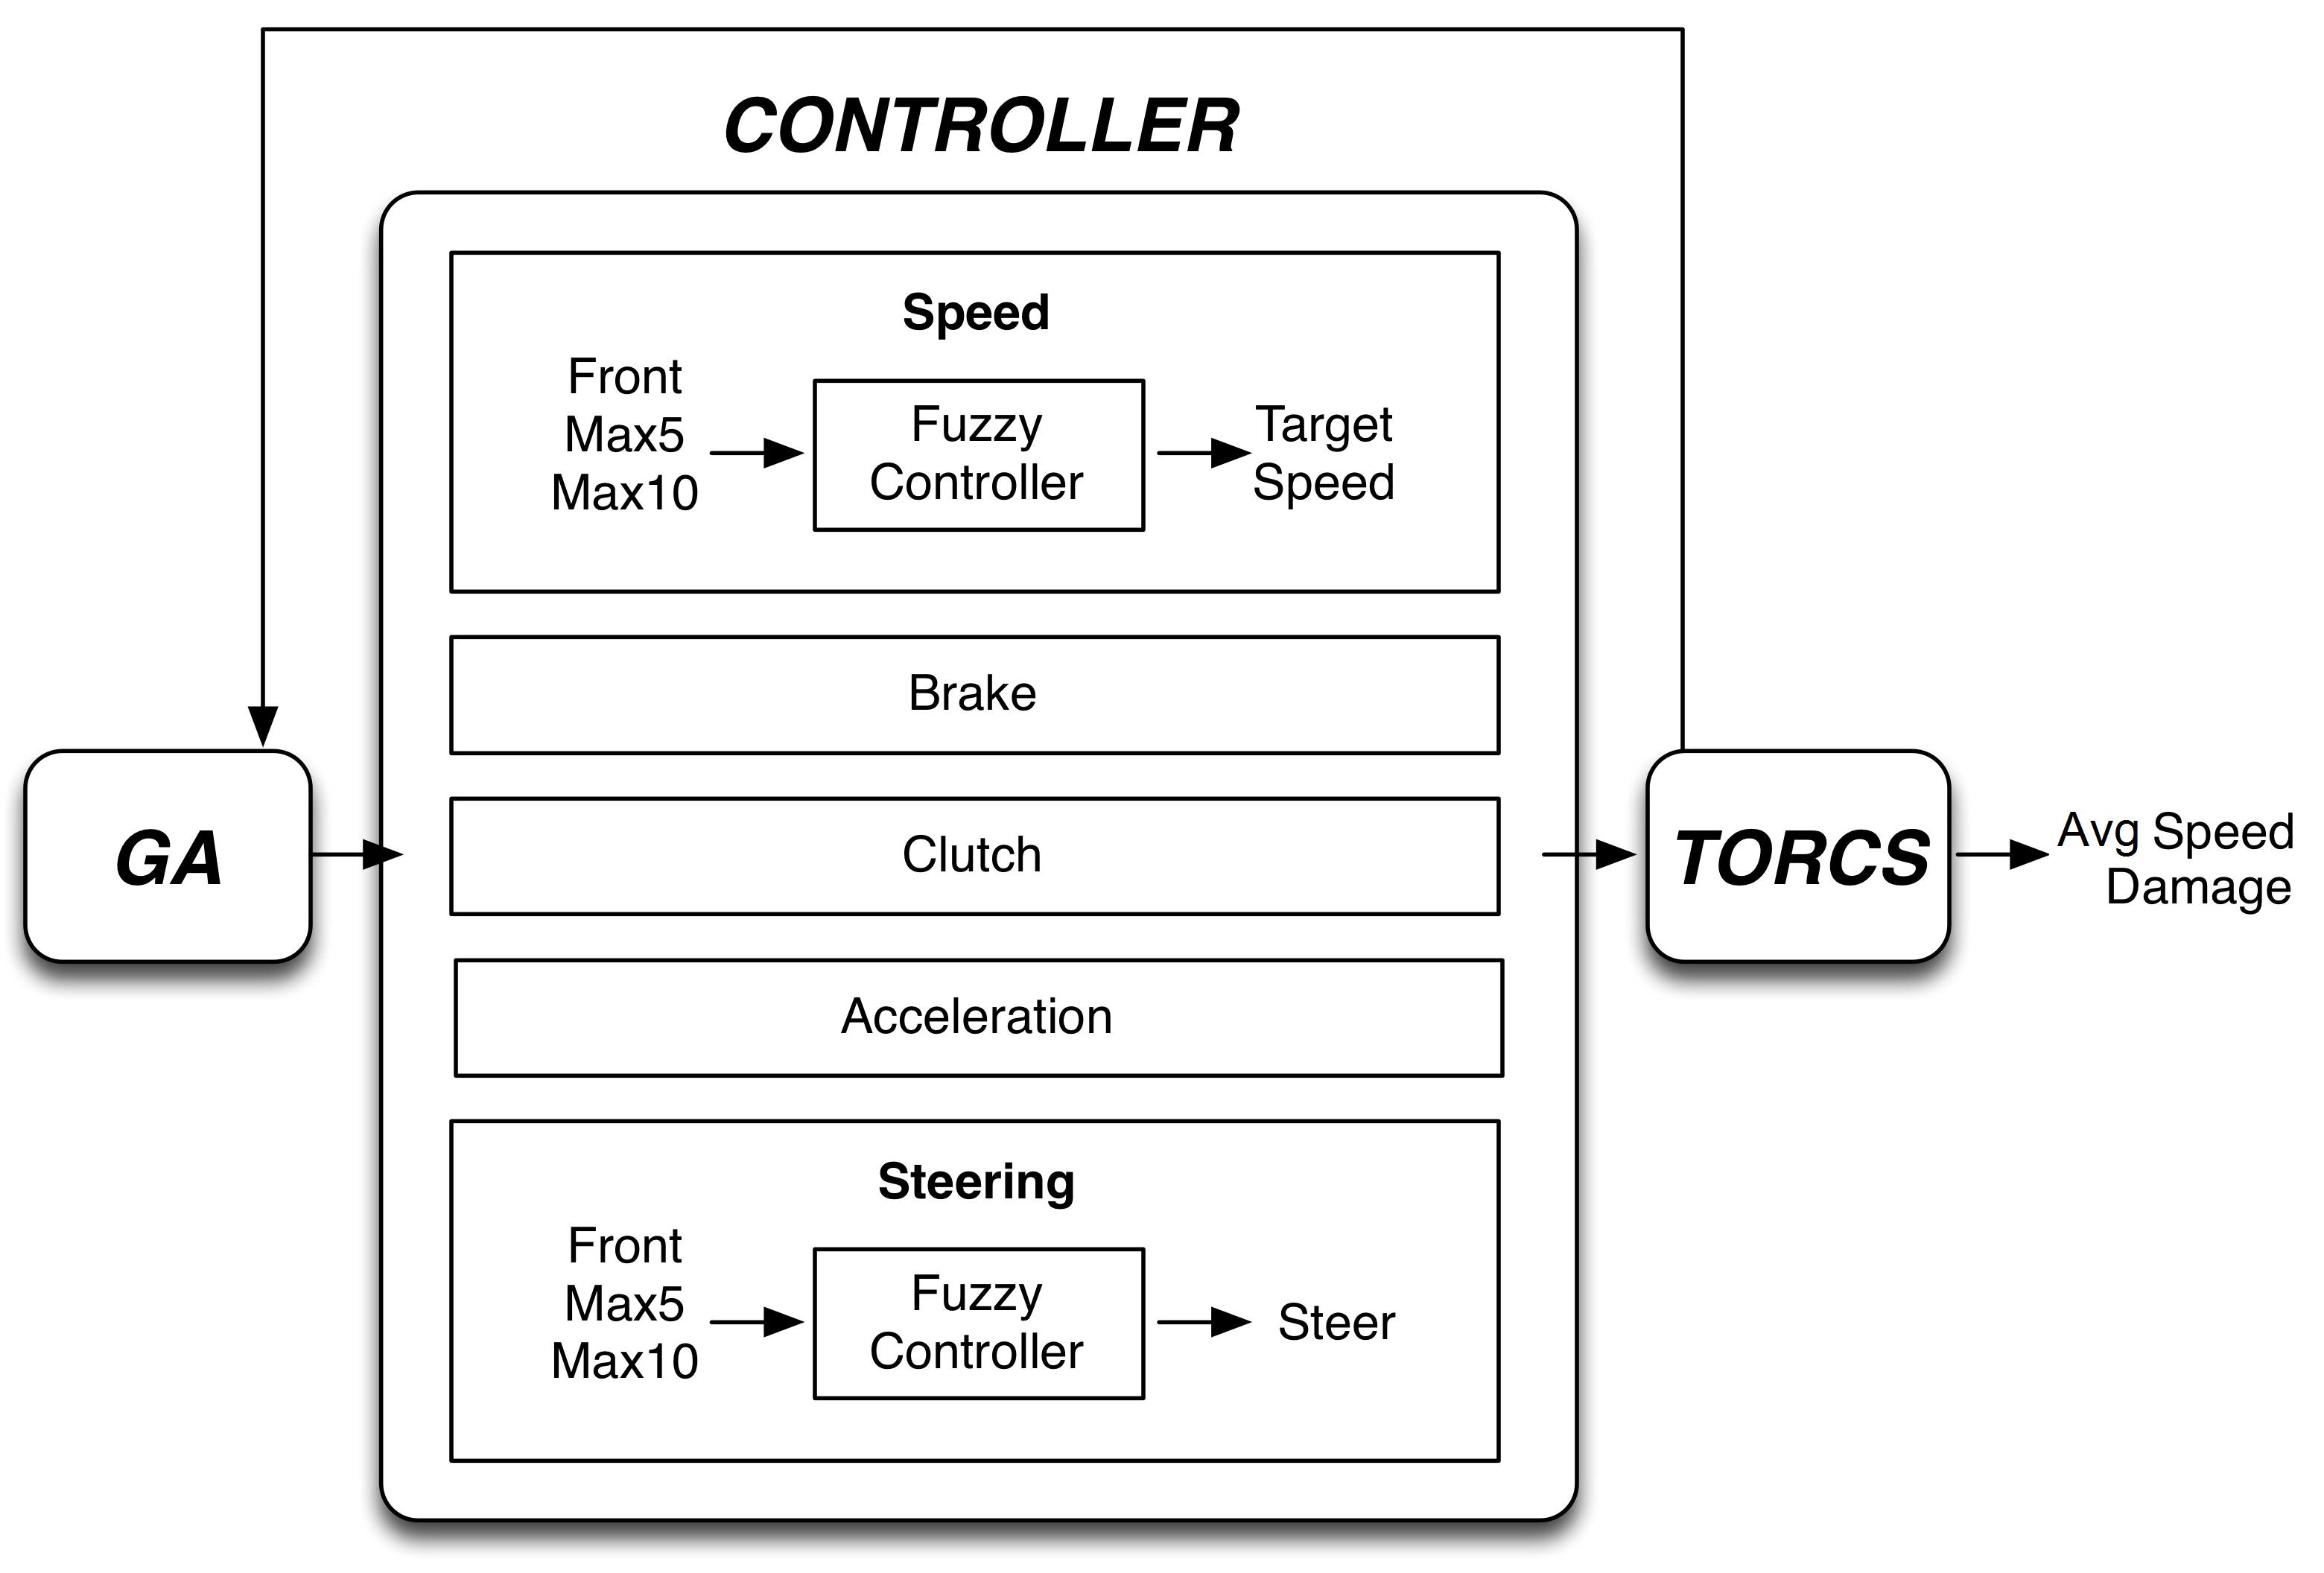
\includegraphics[width=8cm]{fig/flowchart}
  \end{center}
  \caption{Schema of the two GA-evolved controllers evaluated by TORCS, which will
    return the values for the car's average speed on the complete race
    and the incurred damage on the vehicle. Figure taken from
    \cite{salem_evo18}.}
    \label{fig:ga}
\end{figure}
%
The two fuzzy sub-controllers we evolve take care of target speed and steering angle. These controllers were introduced by the authors in a previous paper \cite{salem_evo17}, and share the same structure as the standard TORCS driver but they consider five different sensors (see Figure \ref{fig:torcs-sensors}). These controllers are shown in Figure \ref{fig:ga}. 


The \textit{speed controller} takes as input, sensor values and outputs the target speed; aiming to maximize it, in the straight parts and curves of the circuit. The \textit{steering controller} uses the same sensor values to output the optimal steering angle to reach the desired target position with the car.

The two sub-controllers use the same three linguistic variables as
inputs, one for every sensor: one for the frontal sensor,
\texttt{FRONT}, another for Sensors 8 and 10 ($\pm 5$\textdegree),
\texttt{MAX5}, and finally from Sensors 7 and 11 ($\pm
10$\textdegree), \texttt{MAX10}. These variables compose a Mamdani-based fuzzy
system \cite{iancu2012} with three trapezoidal Membership Functions
(MFs) for each variable. The controller uses a set of fuzzy rules
which combine the fuzzy values for these inputs to compute outputs:
target speed or steering angle.
These rules were designed following the usual human-like race car driving
rules in \cite{salem_evo18}, are fixed and shown in Table \ref{tab:output}.


\begin{table}[h!tb]
  \centering
  {\scriptsize
    \caption{Rules  (from \cite{salem_evo18}) for speed (top) and steering
      (bottom) controller output. Additionally, when 
      the front, right and left sensors have the maximum value
      possible, a crisp rule that tries to set the max speed
      fires.  Angles will be reversed
      if the M10 is equal to Track 7 in the steering controller. The
      actual output will be the centroid of the output of all functions
      that are activated. \label{tab:output}}
    \begin{tabular}{|c|c|c||c|}
\hline
      Value FRONT & Value MAX5 & Value MAX10 & Target Speed (km/h) \\
      \hline
      High & - & - & 280 \\
      Medium & - & - & 240 \\
      Low & High & - & 220 \\
      Low & Medium & - & 180 \\
      Low & Low & High & 120 \\
      Low & Low & Medium & 60 \\           
      Low & Low & Low & 30 \\     
\hline
%\end{tabular}
%\begin{tabular}{|c|c|c||c|}
\hline
      Value FRONT & Value MAX5 & Value MAX10 & $sin$(Steer Angle) \\
\hline
      High & - & - & 0 \\
      Medium & - & High & 0.25 \\
      Medium & Medium & Medium & 0.25 \\
      Medium & Low & Medium & 0.5 \\
      Low & - & High & 0.5 \\
      Low & Medium & Medium & 1 \\
      Low & Low & Medium & 1 \\ 
      
\hline
\end{tabular}
}
\end{table}



Thus, what will be evolved with the algorithm proposed in Section
\ref{sec:ga} is the shape of the whole fuzzy system, which is encoded
in 18 real-valued parameters (related to the different membership
functions). The low-level details of this part were explained
extensively in \cite{DBLP:conf/cig/SalemMG19}. 

As mentioned, these fuzzy sub-controllers proved to be a good platform for the evolution of racing car controllers, and have not essentially changed since our first paper. As a matter of fact, the methods presented in this paper could
be applied to any kind of controller, as long as it can be fully
encoded and evolved using an Evolutionary Algorithm. 

%%%%%%%%%%%%%%%%%%%%%%%%%%%%  OPTIMISING WITH GAS  %%%%%%%%%%%%%%%%%%%%%%%%%%%%
\section{Optimizing Sub-controllers with an Evolutionary Algorithm}
\label{sec:ga}

We have applied an evolutionary algorithm (EA) \cite{EAs_Back96}, to optimize the parameters of the membership functions of the fuzzy sub-controllers we have used in this line of research.
EAs are nature inspired methods that evolve populations of possible (encoded) solutions for a problem following a process of selection of the best,
recombination, and mutation, to create a new population of better individuals on average. This is repeated a number of times
(generations) to get to a solution that meets our requirements, or the
budget we have for evaluation of solutions. EAs have been widely
applied to solve a huge amount of optimization problems, including regression and fuzzy systems \cite{hoffmann2001evolutionary}; in this kind of problem the solutions are modeled as a vector of numeric values, as is the
case in this paper; we use 18 floating-point values, 6 per variable, 2 values per membership function.

Following standard implementations in the first step of the algorithm \cite{salem_evo18} a
population of random individuals is composed by assigning diverse values inside a feasible range ($[0,100]$).

In general, an evolutionary algorithm will need to evaluate every
individual so that they can be compared with each other and decide
which ones will go ahead to the next generation. We use TORCS for this
purpose, as is shown in Figure \ref{fig:ga}: out of the encoded fuzzy
MF values we create a controller, that is assigned to the car, but the evaluation is done in two different ways.

The first method considers the fitness function already used
previously \cite{salem_cig2018}, because it was the most successful 
among some others proposed \cite{salem_evo18}. It is described as: 

 \begin{equation} \label{fit_avg}
 	\begin{array}{lll}
 		f_{AVS}= \frac{AVG(Speed)}{Damage+1}
 	\end{array}
 \end{equation}	

Where $AVG(Speed)$ is the average speed of the car along the complete
race. This factor represents the overall performance of the controller
combining difficult (e.g. curves) and easy (e.g. straight) parts of
the tracks. $Damage$ value is taken into account in order to preserve
the car integrity, which is required to finish the race. 

Following the usual recommendations in the literature
\cite{Harik-ParameterLess99}, we have defined a parameterless
selection method, where there are no weights in the terms.  At the
same time, this way of evaluating different cars is closer to a
`human-like' approach, since it gives the factors the same importance
a human driver would do.

That fitness is computed in a solo race with 20 laps in the chosen circuit. In this paper, however, we also introduce the Grand Prix Selection or GPS. In this
selection, a controller is evaluated in terms of races with the rest
of controllers in the same generation. Fitness is then not
computed directly from telemetry in a solo race, but out of the score
obtained in a championship with several races, where every controller
in a generation participates. This will be described more extensively
in the next subsection.

\textbf{Non-uniform} mutation \cite{mutation1997} has been used as the
\textit{mutation operator} in the GA because it was considered in
previous approaches of our controllers.

The next section describes the two methods we are presenting in this
paper: a competition-based selection policy and an extended real-value
crossover operator to manage the balance between exploration and
exploitation during the evolution.

% -------------------------------------------------------------------
\subsection{Grand Prix Selection and decreasing-$\alpha$ BLX blending crossover operator}
\label{subsec:novel_operators}

As introduced in the previous subsection, the \textbf{Grand Prix
Selection} policy (GPS) aims to select, in every generation, more
reliable individuals/controllers as parents to combine their genes for
creating new individuals in the following generation of the algorithm,
as well as use them as a basis for exploration of new solutions. It is
a competition-based approach, independent of the aforementioned
fitness function (see Equation \ref{fit_avg}), designed to better deal
with the uncertainty present in the election of an actual good
individual using solo races, which is a good surrogate for the actual
objective of evolution, winning competitive races, as has been proved
in our papers so far. However, in this paper, we will examine if using
real races for evolution can be a better option in terms of
performance, and also of evaluation budget.

The mechanism arranges groups of 10 individuals/controllers which are placed in a track in TORCS, where different races are simulated. Thus, they compete, using the same car (i.e. in the same conditions) during several laps. After every race, the controllers get a score according to their position in the final rank. This is a \textit{score function} based on Formula 1 Grand Prix ranking, so the obtained scores per rank are: rank 1 - 25 points, 2 - 18, 3 - 15, 4 - 12, 5 - 10, 6 - 8, 7 - 6, 8 - 4, 9 - 2, 10 - 1.
Then, the best individuals will be those whose accumulated score (sum of scores of all races) are the five highest.

The objective of this operator is to select the best
individuals of the population. However, given the existing uncertainty
\cite{DBLP:journals/tcci/MereloLFGCCRMGTCC16} due to the competition
against other non-deterministic controllers, it is not possible to
ensure they are doubtlessly the best. We claim that this operator will
provide more competitive and reliable individuals than one based on a
`standard' fitness function, since their score just depends on their
ability to win the race against other competent controllers, rather
than in the combination of a set of variables which might add `noise'
to the valuation of the individuals.

However, the application of this method consumes much higher computation time, so it could be combined with a classical fitness-based selection in some generations. Indeed, in the experiments conducted in Section \ref{sec:results}, we have analyzed the impact of the application of different configurations of GPS, considering different frequencies of application during the evolutionary process.

The second operator implemented in our GA is the Blend Crossover or \textbf{BLX-$\alpha$ Crossover} \cite{blx2008} and adapted here to use a varying $\alpha$ value. As stated before, one of the side effects of uncertainty is its derived higher diversification factor. Thus, in order to have better control between the exploration and exploitation factors during the evolution, the balance changes with the decreasing value of $\alpha$.

It is based on the random selection of values from the interval
$[x_i-\alpha(y_i-x_i).. y_i+\alpha(y_i-x_i)]$, where $x_i$ and $y_i$
are the $i^{th}$ values of the parent solutions $x$,$y$ and
$x_i < y_i$. % See Figure \ref{fig:blxalpha}.


Thus, this crossover method was designed for real-coded EAs \cite{blx2008} and creates the offspring (i.e. individuals of the new generation) of the current population by selecting random values for every gene around an interval for each of the parents' genes. So, it can create three new individuals from one parent, which are different between them and, of course, different from their parent individual. This fact enhances the exploration factor in new generations.

The value of the $\alpha$ parameter regulates the exploration/exploitation priority when searching the space of solutions; a value $\alpha = 0.5$ will balance them.

Given the characteristics of an evolutionary algorithm and the way it works, the first generations should be devoted to explore the search space looking for promising areas (those with potential good solutions) where parts of the population could be focused. This would be done through diversification in the individuals.Then, an exploitation process would be recommended, to refine the promising solutions to get to an optimal one.

To this end, we have implemented an \textit{BLX} operator with a decreasing $\alpha$ value, following
the expression: \mbox{$\alpha =1-\frac{g}{g_{max}}$}, where $g$ is the
current generation and $g_{max}$ is the maximum number of generations.

This will mean a higher diversification factor in the first generations because the offspring will take much more different values for their genes in comparison with their parent and other descendants. 
On the contrary, as the number of generations is increased, $\alpha$ will take a smaller value, the intervals will be reduced, the individuals will be more similar to their parents, and thus, the space of solutions will be exploited (the solutions will be refined).

We argue that this operator, in conjunction with GPS will aid the
algorithm to find better controllers, so we will test several
combinations and configurations of both techniques in the experiments
conducted in the next section. We will also study their impact, both considering their performance and also from the uncertainty influence point of view. 
%%%%%%%%%%%%%%%%%%%%%%%%%%%%  RESULTS  %%%%%%%%%%%%%%%%%%%%%%%%%%%%
\section{Experiments and results}  
\label{sec:results}

\begin{figure}[!ht]	
\centering
\begin{subfigure}[b]{0.15\textwidth}
	\centering
	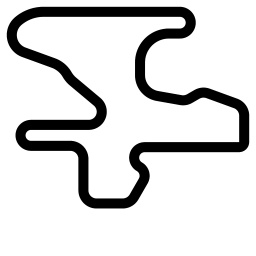
\includegraphics[width=2.5cm]{fig/alpine2.jpg}
%	\caption{Alpine 2 Track.  Length: 3773.57m, Width: 10m.}
	\label{fig:alpine2}
\end{subfigure}
\hfill
\begin{subfigure}[b]{0.15\textwidth}
	\centering
	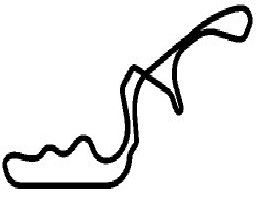
\includegraphics[width=2.5cm]{fig/wheel2.jpg}
%	\caption{\textcolor{red}{Wheel 2 Track.  Length: 6205.46m, Width: 12m.}}
	\label{fig:wheel2}
\end{subfigure}
\caption{Training tracks. Left: Alpine 2; Right: Wheel 2.}
\label{fig:alpine2_wheel2track}
\end{figure}

In this kind of problem, it is essential to select the correct
training track so that bots can work in a wide range of
conditions. Since using several tracks would make evaluation too onerous, we chose to select two tracks to train our solution. The first track is \textit{Alpine 2} track, the one already used in several papers  \cite{salem_cig2018,DBLP:conf/cig/SalemMG19}. This circuit has several characteristics that
are essential for evaluating a bot: it has many turns, some of
them with 180 degrees, steep segments, and some very challenging parts
like the entrance of a tunnel at a square angle. These features make
it a good testbed for good turning and collision avoidance
strategies. Moreover, it also offers a few straight segments which allow the car to speed ahead, reaching high speeds. This same track has been also repeatedly used by other authors for training as well as for testing \cite{cardamone2010applying}, and has been described as ``technical and complex'' \cite{AG} and ``presenting a challenge even at low speeds'' \cite{vrajitoru2018global}; in \cite{AG} it had the third lowest lap time, after \mbox{Alpine 1} and Olethros, implying it has got a good balance between hardness and speed. Since we also used it in our previous papers, it allowed us to compare racing bots that had been ``trained'' in the same conditions.

\mbox{Alpine 2} track is probably one of the most popular tracks used for
training; \mbox{CG-Track 2} has similar features, and it is used by
\cite{mirus2019short,8833873,verma2018programmatically},
in this last case for transfer learning. There are several differences between \mbox{CG-Track 2} and \mbox{Alpine 2}, the one we use, but the main one is that turns are relatively easier and straight segments are longer, favoring fast cars over balanced ones; this is why we have chosen Alpine 2 for training, since
it offers the best generalization for cars trained using it.\\
The second circuit is the \mbox{Wheel 2} Track. It is a  Suzuka F1 track that combines many challenges such as  high-speed parts and different  curve types. Moreover, the eleventh turn is a hairpin turn. It was  described in \cite{wheel2track_chen} as `a more difficult track with many fast turns' (See Figure \ref{fig:alpine2_wheel2track}).
To test the obtained controllers, we considered two tracks: the first track is \mbox{\textit{E-Track 5}}, used in previous papers \cite{salem_evo17},\cite{salem_evo18} and the second one is \mbox{\textit{Street 1}}.
This controller has many long speed segments, difficult sharp turns. In addition, the track is two meters larger than the  other  three considered tracks which  increases the overtaking possibilities.

We have again used the vehicle \mbox{\textit{car1-trb1}},
which is a well balanced, NASCAR type car \footnote{See description in
  the TORCS racing board web page,
  \url{http://www.berniw.org/trb/cars/car_view.php?viewcarid=5}},
which we have used also in our previous papers, and also by many
winning bots  along with the history of the TORCS championship
\cite{torcs5} as well as other authors in the literature
\cite{auteur2010}. This matches well the selection
of racing track, but being as it is a balanced car, allows driving to
fit itself to our developed controllers.


%%%%%%%%%%%%%%%%%%%%%%%%%%%%%%%%%%%%%%%%%%%%
To analyze the influence of the new introduced Grand Prix Selection
(GPS) and the crossover operator on the performance of the fuzzy
controller, we have carried out two main optimization processes based
on the GPS: the first one uses the GPS with the two point crossover
operator while the second uses  BLX with decreasing $\alpha$.
In every process, three controllers are obtained depending on the application of the GPS: in every generation (E), every 5 generations (5), and in the last generation(L). The acronym VA  stands for "varying $\alpha$" in the names of  controllers with BLX and decreasing $\alpha$.
Hence, we experimented with six controllers in all: the new
proposed controllers {\sf GFC-GPSVAE} and {\sf GFC-GPSE}, our previous four GPS based controllers \cite{DBLP:conf/cig/SalemMG19}: {\sf{GFC-GPS5}}, {\sf{GFC-GPSL}},{\sf{GFC-GPSVA5}} and {\sf{GFC-GPSVAL}}.
Also and for comparison purpose, two reference controllers have been considered: {\sf{GFC-VA}}\cite{DBLP:conf/cig/SalemMG19} and {\sf{GFC}}\cite{salem_cig2018}, they both use the fitness function $f_{AVS}$ (Equation \ref{fit_avg}) value for selection.
All these controllers are summarized in Table \ref{tab:drivers}. 


We have run the algorithms with a population size of 60
individuals. The rest of the parameters are: Generations=50, Crossover
rate=0.85, Mutation rate=0.09, and 10 different runs per
configuration.  For every optimization's race, the track is selected
randomly from Alpine2 and Wheel 2 tracks.  We kept the same values for
the evolutionary parameters as in our previous works for two reasons:
first, because they yielded good results (and are not the focus of
this paper), and second, in order to compare previous controllers with
the new ones in the same conditions.


%%%%%%%%%%%%%%%%%%%%%%%%%%%%%%%%%%%%%%%%%%%

\begin{table*}[!htp]
	\centering
	{\scriptsize
		\caption{ Description of the controllers tested in the experiments.}
		{
			\begin{tabular}{|c|c|c||c|}
				\hline
				Controller&Fitness & GPS frequency&Crossover operator \\
				\hline
				\hline
{\sf{GFC-GPSE}}&Competition-based&Every generation&Standard crossover\\
{\sf{GFC-GPSVAE}}&Competition-based&Every generation & Varying BLX$-\alpha$\\

{\sf{GFC-GPS5}}\cite{DBLP:conf/cig/SalemMG19}&Hybrid&Every 5 generations&Standard crossover\\
{\sf{GFC-GPSVA5}}\cite{DBLP:conf/cig/SalemMG19}&Hybrid&Every 5 generations & Varying BLX$-\alpha$\\

{\sf{GFC-GPSL}}\cite{DBLP:conf/cig/SalemMG19}&Hybrid &Last generation &Standard crossover\\

{\sf{GFC-GPSVAL}}\cite{DBLP:conf/cig/SalemMG19}&Hybrid &Last generation & Varying BLX$-\alpha$\\
{\sf{GFC}}\cite{salem_cig2018}& Fitness $f_{AVS}$ (Equation \ref{fit_avg})&-&Standard crossover\\
{\sf{GFC-VA}}\cite{DBLP:conf/cig/SalemMG19}&Fitness $f_{AVS}$ (Equation \ref{fit_avg})& - & Varying BLX$-\alpha$\\


\hline
			\end{tabular}
		}\label{tab:drivers}
	}
\end{table*}
%

% ---------------------------------------------------------------------------

\subsection{Uncertainty in fitness evaluation}

We need first to find out how different  kinds of selection procedures
affect uncertainty in scores (fitness values). Better selection procedures should be able to reduce it, making evolved controllers as centrally distributed
as possible; other kinds of selections should keep  the distribution of
scores (for a single controller) skewed and lopsided; this is why we
have done a study of the distribution of the genetic individuals of
three approaches: {\sf GFC}, {\sf GFC-GPSE}, and {\sf GFC-GPSVA5}. 


Skewness is related to how symmetric the distribution of fitness
scores is. Several strategies deal with this kind of
uncertain (usually called {\em noisy}) fitness functions; but a simple
one is to re-evaluate ({\em re-sample}) the score every generation. A
skewed distribution means that it will more likely to sample a value
that is different from the average, but it might be better or worse
than average; in any case, different from the (crisp) score we would expect to
achieve in other circumstances. On the other hand, kurtosis measures
the number of values that are far from the average, creating either a
heavy-tailed or too-lightly-tailed distribution. In the first case, it
will mean that values far from what would be expected (the median or average) are likely to
show up in the fitness score.

This is why we are interested in how these two statistical measures
are going to change with evolution using the different fitness measures; skewness and kurtosis will  affect the selectability of an individual, so that, in general, most selection procedures will select
individuals with lower kurtosis and skewness, since they are more
likely to draw a consistent value and thus go ahead to the next
generation. However, different selection procedures will affect them
in different ways. This is why we have computed
  skewness and kurtosis for a sample of 20 from the 60 individuals of
  the population evaluated for 50 generations, and measured fitness
  values after the first, the 30th, and the last generation for the three controllers; we take 30 measures of the
  fitness, generating a statistical distribution for the fitness
  values for every individual in the population; what we plot in
Figure \ref{fig:gfcsk} (top, middle, bottom) is the
  skewness and kurtosis of the fitness for every one of these
  individuals. The normal distribution would have skewness and
  excess kurtosis exactly equal to 0.

\begin{figure}[ht]	
	\begin{center}
		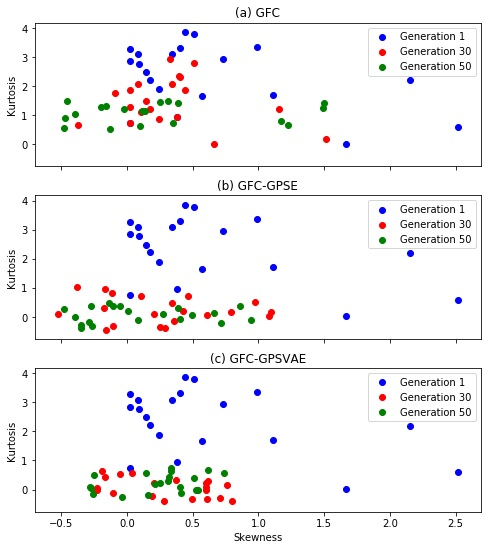
\includegraphics[width=6cm, height=7cm]{fig/skew1.jpg}
		\caption{Excess skewness ($y$) and kurtosis ($x$)
			for the $f_{AVS}$ fitness in the  {\sf GFC} method \cite{salem_cig2018} (top), GPS score in {\sf GFC-GPSE} (middle) and {\sf GFC-GPSVAE} (bottom).}
		\label{fig:gfcsk}
	\end{center}	
\end{figure}
The figures show that the evolution process has a certain influence in
these measures, with individuals in the latest stages of evolution
getting their values closer to the origin, which would be a 0-skewness, 0-kurtosis
Gaussian. However, there are differences between the fitness-based
process ({\sf GFC}) and the other two, which are based on their
performance against other players. This is not only because what we are measuring, is a different value (fitness vs. selection score).
In the first case, the
selection procedure simply eliminates the outliers with a high
skewness or kurtosis; there does not seem to be a big change from
generation 30 to 50, so individuals with high
and skewed variability are selected as {\em winners} when in fact they
are possibly not.

The two methods that use competition for selecting individuals, {\sf
  GFC-GPSE} and {\sf GFC-VA-GPSE}, are
notably similar, with selection eventually making the score of
individuals close to a Gaussian distribution, although slightly skewed
to the right, and with a positive fat tail. However, {\sf GFC-GPSVAE} can find solutions with lower skewness, always between -0.5 and
1. Since this method exploits more found solutions, it seems that it
is able to generate new solutions with a more reliable expected value
around the middle of the area the variable covers, but decreasing more
slowly towards values away from the center. For the time being, we can
affirm that methods that use competition outcomes for selection tend
to evolve individuals with a less uncertain score, and thus more
robust and whose expected
results are more reliable; this was an objective of this GPS
procedure, and we consider it has been achieved, as it can be seen in
Figure \ref{fig:gfcsk}: this last method reaches the minimal
dispersion of skewness in the 50th generation, with kurtosis in a
distribution that is similar to {\sf GFC-GPSE}, but in either case
with lower variability than the one found in the original {\sf GFC} algorithm. Although we have
represented a single run here, results for other runs are similar.

In the next subsection, we will see how this kind of selection has an influence on success as a method for finding high-performance controllers.


% ---------------------------------------------------------------------------

\subsection{Testing Grand Prix Selection and BLX-$\alpha$ controllers}

Once the 10 runs have finished, the best controllers obtained from the
previous evolutionary processes compete again in a similar set of
races, to choose the best controller overall per approach,
i.e. the best between {\sf GFC-GPSL}, {\sf GFC-GPSE} and {\sf
  GFC-GPS5}; and also between {\sf GFC-GPSVAL}, {\sf GFC-GPSVAE} and
{\sf GFC-GPSVA5}. The same F1 Grand Prix score used in GPS selection
is considered. We run the selected controllers in 10 races of 20 laps
for each of the two training tracks: Alpine 2  and Wheel 2  and  for
each of the two testing tracks: E-Track 5 and Street 1. Results are
shown in Table \ref{tab:GPS_and_Varyingalpha_RSresults}.

The main intention of these experiments is to
  highlight the differences in performance brought by the different
  operators and methods used, as well as establishing a new state of
  the art in TORCS. We use 10 controllers in every experiment, since
  this amount of cars, will create conditions that will show the
  quality of the controllers avoiding collisions or overcoming other
  cars. The fact that some controllers in every set of races are theoretically similar (due to the fact that only one operator or selector changes from one to the next) will not be a problem, but rather a way of highlighting the clear differences in
  performance, as we will see later.



\begin{table}[h!]
	\centering
	{\scriptsize
		\caption{ Results of GPS controllers and varying $BLX-\alpha$ controllers in a mini-championship with 10 controllers and 10 races in two different training tracks and two testing tracks (20 laps each). {\tt tita}, {\tt berniw}, and {\tt	inferno} are example controllers included with TORCS \cite{torcs4}. In {\bf boldface} the best value, and in {\em italics} the second best.}
		{
                  \begin{tabular}{|c|c|>{\columncolor[gray]{.9}}c|c|c||c|}
                  	              \hline
                  	\multicolumn{6}{|c|}{Results of GPS controllers} \\
                    \hline
                    
%                    \rowcolor{gray!30}
                    & \multicolumn{2}{|c|}{Training tracks} &\multicolumn{2}{|c|}{Testing tracks}& \\
                    \hline
                    Controller&\textit{Alpine 2} &Wheel 2&\textit{E-Track 5}  &Street 1&Total\\
				\hline
				\hline
			
			{\sf GFC-GPSE}&216& 222& 236&222&{\bf 896}\\	
			{\sf GFC-GPS5}\cite{DBLP:conf/cig/SalemMG19}&170&162&176&180&{\em688}\\
			
			{\sf GFC-GPSL}\cite{DBLP:conf/cig/SalemMG19}&164&154&156&156&630\\
			{\sf GFC} \cite{salem_cig2018}	&140&116& 86&114&456\\
			{\sf GFC-VA}\cite{DBLP:conf/cig/SalemMG19}	&102&102& 68& 90&362\\



			$berniw2$	& 84&100&100& 72&356\\
			$tita1$	&44 & 64& 58& 60&226\\
			$inferno2$&50& 34& 72& 50&206\\				
			$berniw1$	& 24& 26& 42& 52&144\\			
			$inferno1$& 16& 30& 16& 14& 76\\			
			
				\hline
              \hline
               \multicolumn{6}{|c|}{Results of varying $BLX-\alpha$ controllers} \\
                            \hline
              \hline
                    Controller&\textit{Alpine 2} &Wheel 2&\textit{E-Track 5}  &Street 1&Total\\
              \hline
              \hline	
              {\sf GFC-GPSVAE} &236&	236&250&236&{\bf 958}\\
              {\sf GFC-GPSVA5} \cite{DBLP:conf/cig/SalemMG19}&170&	188&162&188&	{\em 708}\\

				{\sf GFC-GPSVAL} \cite{DBLP:conf/cig/SalemMG19}&152&	156&146&	156&	610\\

				
				
		{\sf GFC-VA} \cite{DBLP:conf/cig/SalemMG19}&124&96 &102&	108&	430\\		
		{\sf GFC}  \cite{salem_cig2018}&102&	96 &88 &	100&	386\\
		$berniw2$	 &76 &	88 &74 &76 &	314\\
		$tita1$	 	&52 &60 &56 &	56 &	224\\
		$inferno2$ &40 &	44 &80 &	24 &	188\\		
		$berniw1$	 &36 &	24 &30 &	48 &	138\\	
		$inferno1$ &22 &	22 &18 &18 &	80\\					\hline			
			\end{tabular}
		}\label{tab:GPS_and_Varyingalpha_RSresults}
	}
\end{table}
%
As Table \ref{tab:GPS_and_Varyingalpha_RSresults} (top subtable)
shows, the controller {\sf GFC-GPSE} has won the Grand Prix
championship obtaining 438 points from 500 in the tracks used during
training; it has also ranked first in the testing tracks
\textit{E-Track 5} and \textit{Street 1}.
The other GPS based controllers have obtained nearly the same results (149 and 158 respectively).
From the same subtable, it is clear that the controller {\sf GFC-GPSE}, where GPS selection has been applied in every generation, has won the majority of possible points in the four tracks, even in the unknown (not trained) \textit{E-Track 5}  and \textit{Street 1} tracks.

These results come to confirm the influence of the proposed selection policy where the controllers obtained from applying only the GPS selection have won the competition (comparing the points obtained by GPS controllers and GFC).
Indeed, we have made a `realistic' selection process by eliminating
the classical fitness function based on the speed and damage average
and replacing it by points obtained in direct races. 
Performance in solo racing can be an acceptable criterion for a good
controller, as proved so far, but at the end of the day, the best car
is the one that wins races. Thus, the new selection policy allows us
to select actual winners on the field and not controllers that perform
well in {\em training} races and could, thus, be potential winners.

% ----------------

The next experiment is dedicated to assess the impact of the
$BLX-\alpha$ operator; the same process has been followed
selecting the best controllers of the evolution from those which
have used this varying-$\alpha$ crossover operator and testing them in several
races. Results are shown in Table \ref{tab:GPS_and_Varyingalpha_RSresults} (bottom subtable). 


As it can be seen in the table, again the controller using GPS in
every generation has reached the best score, but it should be noted the
big impact of the application of the varying $BLX-\alpha$ operator in
all the controllers. Thus, looking again at the results in Table \ref{tab:GPS_and_Varyingalpha_RSresults} (bottom subtable) 
and comparing them with those in the top subtable (results of GPS controllers), the increase in the obtained score is evident, at least in the first
two. 
Thus, the introduction of the $BLX-\alpha$ operator allows the parameters of the controllers to be refined and increases diversification in the optimization process, which has led to better results.
Finally, the best controllers obtained from the two main optimization
processes: {\sf GFC-GPSVAE} and {\sf GFC-GPSE} are evaluated in an F1 like mini-championship against the previous five TORCS bots and the {\sf GFC-VA}\cite{DBLP:conf/cig/SalemMG19} and {\sf GFC} controllers  \cite{salem_cig2018}. 



We have also considered a new rival from the state of the art, which participated in several Simulated Car Racing Competitions in past editions. 
It was proposed by P{\'e}rez-Li{\'e}bana, S{\'a}ez, Recio, and Isasi, and improved in the work \cite{PerezEvolvingFuzzy09}. We have baptized it as \textit{PSRI} in honor of its authors' surnames. 
Table \ref{tab:allsresults} shows the obtained results.
%

\begin{table}[ht]
  \centering
  {\scriptsize
    \caption{ Results of {\sf GFC-GPSVAE} and {\sf GFC-GPSE}
      in a mini-championship with 10 controllers
      and 10 races in two different training tracks and two testing tracks (20 laps each). {\tt tita}, {\tt berniw}, and {\tt inferno} are example controllers included with the TORCS
      simulator \cite{torcs4}.  {\bf Boldface} is used to highlight
      the best value, {\em italics} for the second
      best. We sort controllers according to the
        overall score, but please note that this ranking need not be
        kept in every column.}
    {
            \begin{tabular}{|c|c|c|c|c||c|}
	\hline
	& \multicolumn{2}{|c|}{Training tracks} &\multicolumn{2}{|c|}{Testing tracks}& \\
	\hline
	Controller&\textit{Alpine 2} &Wheel 2&\textit{E-Track 5}  &Street 1&Total\\
        \hline
        \hline



{\sf GFC-GPSVAE}	&222&236&236&222&	{\bf 916}\\
{\sf GFC-GPSE}	&176&196&162&190&{\em 724}\\

{\sf GFC-VA} \cite{DBLP:conf/cig/SalemMG19}&172&146&	134&152& 604\\
{\sf GFC}  \cite{salem_cig2018}	&108&	120&110&	112&	450\\
$PSRI$\cite{PerezEvolvingFuzzy09}&102&88 &104&86 &380\\
$berniw2$		&88	&84 &92 &72 &336\\
$inferno2$	&58	&34 &80 &50 &222\\
$tita1$		&34 &64 &36 &60 &194\\
$berniw1$		&32	&26 &48 &52 &158\\
$inferno1$	&18	&30 &16 &14 &78\\
\hline

\end{tabular}
}\label{tab:allsresults}
}
\end{table}




This final competition shows {\sf GFC-GPSVAE} clearly leading. It
collected most of the points in the four tracks, leaving the {\sf
  GFC-GPSE} controller far behind it. The reference drivers, namely
{\sf GFC-VA} and {\sf GFC}  are classified $3^{rd}$ and $4^{th}$.

Let it be noted that there are very few individual
  differences in the ranking obtained for individual methods in every
  track; ranking by total score is very similar to rankings in every
  one of the tracks. In the case of our fuzzy-controller based
  algorithms, this shows basically its robustness across different
  track conditions. Also and, in general, published controllers are also robust
  enough to not have big drops in performance in specific
  tracks; sometimes they are subsequent controllers in a series, so
  it is only natural that {\tt berniw2} and {\tt inferno2} are better
  than the first ones in the series. However, among different {\em
    brands}, there are small differences in some tracks: {\sf
    Wheel 2} track makes {\tt berniw1} underperform, for instance; or
  {\sf Street 1}, which makes {\tt inferno1}, with its 36-score
  difference with respect to the second worse {\tt inferno2}, fall to
  last in the overall rankings.

%%%%%%%%%%  controller GFC-VAGPSE MFs

As an additional result, we depict the structure of the winner controller {\sf GFC-GPSVAE} in Figure \ref{fig:frontmfs}. 
If we take into account the rules already set in Table
\ref{tab:output}, the shape of the obtained MFs  is in accordance with
what a human driver would have done: favor speed as much as possible
in the straight sections and brake as late as possible in the turns. 
According to the figures, we have more than three-quarters of the probability that the first three rules will activate; these rules
would make the car very aggressive especially in the straight sections
of the track. The MFs for the FRONT sensor are for most of the values
either Medium or High, which means that the target speed output will
be over 240 km/h for the majority of the sensor range. 
That situation is similar for the MAX5 and MAX10 MFs: turning will be done smoothly, and only in a very extreme situation (with the FRONT sensor in LOW and
the other two sensors or medium or high, it will take a sharp turn;
considering the physics of the simulator, these sharp turns might lead
to getting off track and thus damage to the car.

%
\begin{figure}[h]	
  \begin{center}
    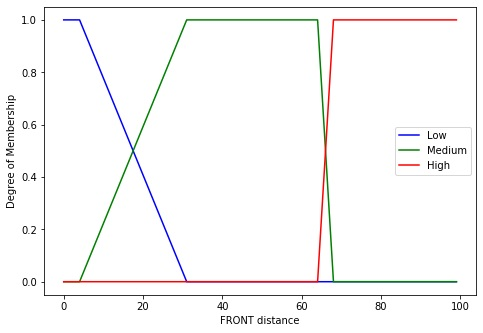
\includegraphics[width=6.5cm, height=1.7cm]{fig/FRONT.jpg}
    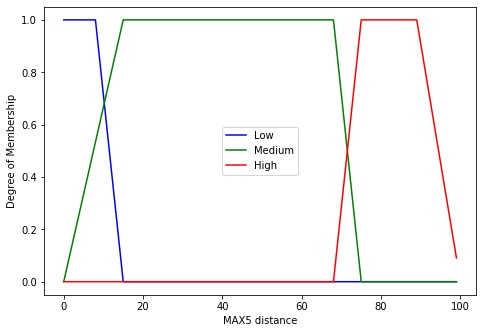
\includegraphics[width=6.5cm, height=1.7cm]{fig/MAX5.jpg}
    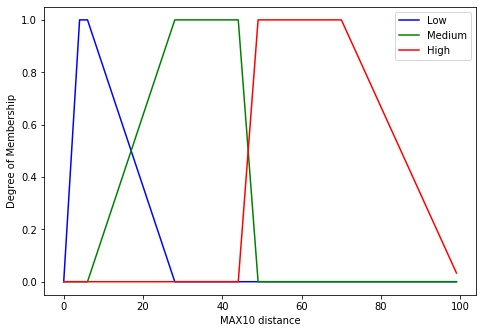
\includegraphics[width=6.5cm, height=1.7cm]{fig/MAX10.jpg}		
    \caption{FRONT, MAX5 and MAX10 input membership functions for a controller obtained with {\sf GFC-GPSVAE} method.}
    \label{fig:frontmfs}
\end{center}	
\end{figure}

Since these MFs lead to very reliable performance in the car, it
validates our approach of using fixed rules. It should
also be noted that the fact that we are using fuzzy controllers allows
us for an easy interpretation of the behavior of the car, something
that would not be possible if other black-box heuristics were used.

%%%%%%%%%%%%%%%%%%%%%%%%%%%%%%%%%%%%%%%%%%%%%%

To evaluate the cost of the proposed controllers, we run the evolutionary optimization for 50 generations and 10 runs for all the considered controllers.
 Table \ref{tab:time} shows the average running time and  as additional information, the range of generations where the best individual was found.

\begin{table}[!ht]
	\centering
	{\scriptsize
          \caption{Average runtime in 10 runs of 10 races 
            and
                  generation where the best individual was spawned.}
		\label{tab:time}
		\begin{tabular}{|p{2.85cm}|p{2.20cm}|p{1.65cm}|}
			\hline  
			Controller& \textbf{Avg Runtime (s)}&\textbf{Generation}\\
\hline
\hline 	 
 \textbf{{\sf GFC-GPSVAL}} \cite{DBLP:conf/cig/SalemMG19}&282923
&7-14\\	
\textbf{{\sf GFC-GPSVAE}}&287200
&11-16\\
 \textbf{{\sf GFC-GPSE}}&289850
&20-39\\
\textbf{{\sf GFC-VA}} \cite{DBLP:conf/cig/SalemMG19}&293000
&9-18\\
 \textbf{{\sf GFC-GPSL}} \cite{DBLP:conf/cig/SalemMG19}&295445
&21-35\\
\textbf{\textbf{{\sf GFC}}} \cite{salem_cig2018}&402000
                   &32-36\\
\textbf{{\sf GFC-GPSVA5}} \cite{DBLP:conf/cig/SalemMG19}&436520
&7-15\\		
 \textbf{{\sf GFC-GPS5}} \cite{DBLP:conf/cig/SalemMG19}&443860
				&21-35\\	
					
			\hline 
		
		\end{tabular}
		
	}
\end{table} 
{\sf GFC-GPSVAE and {\sf GFC-GPSE} controllers were the best where
they are ranked $1^{st}$ and $2^{nd}$ in the comparative competition (See Table \ref{tab:allsresults}) but they are very expensive in runtime } since they have performed around 282923s and 287200s respectively, which is a
huge training time. 
           
This means that, even if the proposed selection policy is very effective, in turn, it requires a lot of computation time.
Another point that we can highlight is that the controllers with
$BLX-\alpha$ have reached the optimal solution in a few generations
(between the $7^{th}$ and the $20^{th}$) while the other methods required more
generations. 
 %%%%%%%%%%%%%%%%%%%%%%%%%%%%
\section{Conclusions and Future Work} 
\label{sec:conclusions}

In this paper, and in order to avoid the impedance between using solo
racing scores and performance in competitive races, we have
incorporated this competition into the selection of individuals in an
evolutionary algorithm that evolves fuzzy controllers in the TORCS
simulator. This selection policy, called GPS (as in Grand Prix
Selection), has been evaluated in combination with hybrid methods that
use it only part of the time, and also together with a varying
BLX-$\alpha$ and standard crossover operators, to assess how it
interacts with them and which combination yields the best competitive
results.
In races performed in the training, and other, tracks, the controller
that has evolved using competitive selection and the
variable-$\alpha$ BLX crossover operator has proved superior to not
only other controllers evolved previously by us, but also other
competitive entries. As a matter of fact, the use of the GPS method has the greatest
influence in the results: {\sf GFC-GPSVAE} and {\sf GFC-GPSE}, whose only
difference lies in the kind of crossover operator they use, create the
best controllers, finishing first and second in competitive races and,
in the first case, obtain twice the score of a non-evolved
competitor such as $berniw2$.

The  BLX operator with decreasing $\alpha$ also has got a positive
influence on the outcome, outperforming the standard crossover
results. Thus, the decreasing amount of exploration that this BLX-$\alpha$ boasts seems to get to areas with better solutions in a
more efficient way, eventually finding very competitive controllers.

Another advantage of these combined selection and crossover operators is that they do not
increase too much the total training time, and are also able to find a
good solution in the first stages of evolution, which, if needed,
allows to cut the training short. {\sf GFC-GPSVAE} needs at most 18
generations (which is around one third of the maximum number of
generations defined) to find a good solution. Running GPS every
generation needs more generations to get to the best that if it is run
every 5 generations, or just at the end, but the problem is that in
those cases the solution found is less competitive. However, {\sf
  GFC-GPSVA5} is quite competitive, and in the case of a limited
evaluation budget, it could be a very good compromise.

As a conclusion, in this paper, we have proved that combining a fitnessless evolutionary algorithm with a varying, floating point,
crossover operator, consistently obtains the best results so far in
TORCS. The sets of choices of running track, car, controller, and actually parts of it that are evolving are thus also validated by
these results. Since the tracks have been specially selected to be as
general as possible, we think that this result could be extended to
other tracks, as long as ``training'' or evolution uses a track that
has as many different features as possible.

We also think that results are probably independent of the fact that
we are using a set of fuzzy controllers, and could be
generalized to any kind of controller, as long as the evolution
process has the possibility to explore the space of controllers in the
same, efficient, way. This is a possible way of extending the work:
substituting fuzzy controllers by simple neural nets could be a way of
proving that the fitnessless approach can find good results
independently of the low-level algorithms using to drive the
car. Fuzzy and neural controllers could be also mixed, even coevolved,
to try and find the best ones. Since the GPS method
  operates at a level that is independent of the type of controller used, by
  reducing uncertainty in the evaluation of a controller, it will likely be able to improve over a baseline controller
  optimization method that would use solo-races for evaluation, although of course no affirmation
  can be made over its performance relative to this one (based on
  fuzzy controllers) or others.

Additionally, we have been using heuristic rules for computing outputs
from the fuzzy rule activation. We could, however, consider optimizing
the outputs of the fuzzy controllers, as well as the rules. The implementation could also be optimized. Right now, training takes
a long time. This optimization could go from parallelization, to basic
program-level improvement.

Robustness in results has been our main objective, but
  we have not really investigated the reason why the fitness
  distribution of controllers in solo races usually has a positive
  skewness, and what could be the reason for this. An interesting
  avenue of research would be to deal with this fact on an individual
  basis and continuing with solo races so that we avoid the big   computational budget we need to perform GPS.

\section*{Acknowledgments}

Supported in part by MINCYT projects
TIN2017-85727-C4-2-P and  RTI2018-102002-A-I00 and project
B-TIC-402-UGR18 (FEDER and Junta de Andaluc\'{i}a).

\bibliographystyle{IEEEtranS}
\bibliography{fuzzy_torcs,geneura,uncertainty,fitnessless}

%\begin{IEEEbiographynophoto}{Juan~J.~Merelo}
%Biography text here.
%\end{IEEEbiographynophoto}


% You can push biographies down or up by placing
% a \vfill before or after them. The appropriate
% use of \vfill depends on what kind of text is
% on the last page and whether or not the columns
% are being equalized.

%\vfill

% Can be used to pull up biographies so that the bottom of the last one
% is flush with the other column.
%\enlargethispage{-5in}



% that's all folks
\end{document}
